\section{Effect of an azimuthal field}\label{result3}
In this section we add an azimuthal field so that $B_y\neq 0$,  
parameterized by $\epsilon \equiv B_y/B_z$. However, we continute to
use $B_z$ for normalizations and $\beta$ is associated with the
vertical Alfven speed. We also extend the previous calculations to the
full disk $z\in[-Z_s,Z_s]$, which allows us to compare the effect of
self-gravity on MRI modes with different symmetries across the
midplane. 

\subsection{Ideal disks with MRI} 
Here we consider an isothermal disk with $Q=0.2$
($Q_\mathrm{2D}=0.72$) and $\beta=10$ in the limit of ideal MHD
($\Lambda_0=100$). Gravitational instability is not expected because 
Fig. \ref{compare_growth3} shows that even for $Q=0.18$, GI is 
surpressed for $\beta \lesssim 15$. We consider azimuthal field
strengths with $\epsilon\in[0,3]$. 

Fig. shows the MRI growth rates for the above system as a function of
$k_x$. The top panel are modes with even midplane symmetry: 
$W^\prime(0)= 0$ for $\epsilon\to0$, and the bottom panel are modes with odd midplane 
symmetry: $W(0) = 0$ for $\epsilon\to0$. The latter set of modes were 
excluded in the previous sections by midplane boundary 
conditions. The plot also include growth rates computed in the Cowling
approximation. As expected,  $\avg{E_g}<\avg{E_m}$, so none of the
modes are energetically dominated by self-gravity. 


%no GI for odd modes 

%general stabilization of MRI

\begin{figure}
  \includegraphics[width=\linewidth,clip=true,trim=0cm 2cm 0cm
    0cm]{figures/compare_growth3_tilted_even.ps}  
  \includegraphics[width=\linewidth,clip=true,trim=0cm 0cm 0cm
    0.52cm]{figures/compare_growth3_tilted_odd.ps} 
  \caption{Growth rates in massive isothermal disks with $Q=~0.2$ and
    $\beta=10$ for a range of azimuthal field strengths $B_y/B_z$. The
    dots are solutions computed from the full problem, with the
    colorbar measuring the gravitational potential perturbation, while
    the solid curves are computed from the Cowling approximation. The
    top panel correspond to even modes and the
    bottom panel correspond to odd modes, which have
    $W^\prime(0)=0$ and $W(0)=0$, respectively, for $\epsilon\to0$.
    \label{compare_growth3_tilted}}
\end{figure}

%We consider $\epsilon\equiv B_y/B_z \in[0,3]$. The 

Consider first the even modes in the top panel of 
Fig. \ref{compare_growth3_tilted}. %Self-gravity slightly stabilizes
%modes with small $k_x$ as $B_y$ is increased. 
Self-gravity destabilizes modes with  $k_xH\gtrsim O(1)$. Consequently, the
cut-off wavenumber is larger when SG is included. %get smaller scale
                                %MRI 
Destablization is most effective for purely vertical fields: with
$\epsilon=0,\, 
k_xH\simeq 1.4$, SG increases the growth rate by $\sim 30\%$. Although
these modes are fundamentally magnetic, this is consistent with
\cite{goldreich65a}, who find SG can only destabilize 
symmetric density perturbations, which is the case for $B_y=0$ here.  
With increasing $\epsilon$, we find the density perturbation $W$ deviates from an even 
function, $|W(0)|$ decreases and $\max{(|W|)}$ moves off of the mid-plane.  
%density pert at the midplane goes down
%We expect this to reduce the destabilization
%effect of SG,  
Together with the increased total magnetic pressure with 
$\epsilon$, destabilization by SG weakens. 
Thus, the Cowling approximation becomes increasingly good with stronger
$B_y$ for the even modes. 

%This destabilization effect weakens with
%$B_y$ because the total magnetic pressure increases, which generally
%opposes GI, although the modes are fundamentally associated with MRI.  

The modes in the bottom panel of Fig. \ref{compare_growth3_tilted} 
display opposite behavior. For $B_y=0$, $W$ is odd and 
self-gravity has no effect. When $B_y>0$, we find $W$ deviates from an odd
function and the mid-plane density perturbation $|W(0)|$ increases. 
SG is stabilizing for these modes at all wavelengths, and is most
effective at $k_xH =  O(1)$.  
%destabilizing effect is absent  
%for $\epsilon=0,\, k_xH\simeq 1.2$, SG decreases the growth rate by $\sim
%13\%$.     

Fig. \ref{result_tilted} show eigenfunctions for $\epsilon=3$ and
$k_xH=1.2$ with and without the Cowling approximation. These differ
from the even modes considered above in that the horizontal magnetic
perturbations maximize at $z=0$ (cf. Fig. \ref{mri_massive_resis}).  
SG significantly enhances the mid-plane density perturbation, making the
gravitational potential energy comparable to the magnetic energy, 
which becomes more confined near the mid-plane. 

\begin{figure}
  \includegraphics[width=\linewidth,clip=true,trim=0cm 1.5cm 0cm
    0cm]{figures/result_tilted_cowling.ps}  
  \includegraphics[width=\linewidth,clip=true,trim=0cm 0cm 0cm
    0.cm]{figures/result_tilted_fullsg.ps} 
  \caption{Energy densities for a MRI mode in an isothermal ideal disk
    with an azimuthal field $B_y = 3B_z$, computed in the Cowling
    approximation (top) and with full self-gravity (bottom). These
    modes correspond to those in the bottom panel of
    Fig. \ref{compare_growth3_tilted}.    
    \label{result_tilted}}
\end{figure}

%strong field, compressibility 
To interpret the above result for odd modes, note 
that compressibility affects the MRI in the presence of an 
azimuthal field, even in a non-self-gravitating disk. If the perturbed 
disk remains in vertical hydrostatic equilibrium, then 
\begin{align} 
  |W|\sim \frac{B_y}{\mu_0\rho}|\dby|,
\end{align}
to order of magnitude in a non-SG disk, so a strong toroidal field can
cause a large density perturbation
\citep{pessah05}. Fig. \ref{result_tilted} shows that this is
amplified by self-gravity.  

We checked that for the modes in Fig. \ref{result_tilted} the vertical
velocity is small, $|\dvz|/\left(|\dvx|^2+|\dvy|^2\right)^{1/2}
\lesssim 0.2$, so the above argument applies. Compressibilty is 
enhanced by both the azimuthal field and self-gravity, which tends
to stabilize the MRI \citep{kim00}. Its effect is important here  
because the azimuthal Alfven speed is sonic. The destabilization
effect of SG is absent (or unimportant) because the density
perturbation is not symmetric.  

%The results for even and odd modes are do not contradict each
%other. Self-gravity tends to be destabilizing, but this requires the
%density perturbation to be symmetric, as is the case for the even
%modes. 
%For the MRI however, compressibility has a stabilizing effect 

%scale separation for odd modes? because modes with kx=1 will be
%quenched 


% for $\beta=10$ and
%$\epsilon=3$. 
%because magnetic energy is concentrated near midplane    
%magnetic pressure, need thermal pressure 
%This
%can subsequently be amplitfied by its self-gravity. 
%That is, compressibility is enhanced by both
%For $\epsilon=3$ and $\beta=10$ the azimuthal Alven speed is
%sonic. Compressibility becomes important for strong toroidal
%fields. If the system remains in approximately vertical hydrod

\subsection{Resistive disks with GI}
Here we examine an isothermal, resistive disk with $Q=0.18$ and
$\Lambda_0=0.1$. GI is permitted, and has a similar growth rate as the
MRI. 



%\subsection{GI}

